\section{Method}
\label{sec:method}

% Fig. 1: training-data pipeline (top) and network (bottom). Pure TikZ, compiles on Overleaf.
\begin{figure*}[t]
\centering
\begin{tikzpicture}[
    font=\footnotesize, >={Stealth[length=4pt]}, node distance=3mm,
    box/.style={draw=black!70, rounded corners=1.5pt, align=center, inner sep=2.5pt, minimum height=9mm},
    data/.style={box, fill=blue!6},
    op/.style={box, fill=orange!10},
    aug/.style={draw=black!50, rounded corners=1pt, fill=orange!10, align=left, inner sep=1.6pt, font=\scriptsize, text width=23mm},
    net/.style={box, fill=green!8},
    lab/.style={font=\footnotesize\bfseries, anchor=west},
    arr/.style={->, thick, black!70}]
% ---------------------------------------------------------------- (a) data
\node[lab] at (-0.55, 1.25) {(a) Training data: offline augmentation, generic (not tuned to the test set)};
\node[data, text width=17mm] (src) at (0.55,0) {12,000 train\\images, $512^2$\\JPEG q95};
\node[aug, right=6mm of src, yshift=4.5mm] (a1) {\textbf{A} brightness, contrast, saturation, hue, gamma, grey};
\node[aug, below=0.8mm of a1] (a2) {smooth-patch blur (label kept)};
\node[aug, right=1.6mm of a1] (b1) {\textbf{B} rescale $\times$0.9--1.1, 5 resamplers};
\node[aug, below=0.8mm of b1] (b2) {flip, rot90};
\node[aug, right=1.6mm of b1] (c1) {\textbf{C} blur $\sigma{\le}0.8$, noise $\sigma{\le}3$};
\node[aug, below=0.8mm of c1] (c2) {JPEG q60--100, 4:4:4/ 4:2:2/4:2:0; 20\% twice};
\node[draw=orange!70!black, dashed, rounded corners=2pt, inner sep=2pt, fit=(a1)(a2)(b1)(b2)(c1)(c2),
      label={[font=\scriptsize, text=orange!50!black]below:$\times10$ copies per image ($\times20$ for the smoothest 25\% of fakes), stored once}] (augbox) {};
\node[data, right=5mm of augbox, text width=17mm] (store) {152k images\\(12k originals +\\140k copies)};
\node[op, right=of store, text width=11mm] (crop) {random\\$256^2$ crop};
\node[net, right=of crop, text width=10mm] (netA) {network\\(b)};
\node[op, right=of netA, text width=10mm] (ce) {cross-\\entropy};
\draw[arr] (src) -- (src -| augbox.west);
\draw[arr] (augbox) -- (store); \draw[arr] (store) -- (crop); \draw[arr] (crop) -- (netA); \draw[arr] (netA) -- (ce);
% ---------------------------------------------------------------- (b) network
\begin{scope}[yshift=-2.75cm]
\node[lab] at (-0.55, 0.95) {(b) Network: NPR input, full-resolution stem, anti-aliased down-sampling (11.17M parameters)};
\node[data, text width=12mm] (x) at (0.3,0) {image $x$\\$3{\times}H{\times}W$};
\node[op, text width=29mm, minimum height=6mm] (npr) at (2.35,-1.05) {NPR residual (0 params)\\$r(x)=x-U_2D_2\,x$};
\node[op, text width=14mm] (cat) at (4.45,0) {$[x;\,r(x)]$, 6 ch\\BN (non-affine)};
\draw[arr] (x) -- (cat); \draw[arr] (x.south) |- (npr.west); \draw[arr] (npr.east) -| (cat.south);
\node[net, right=3mm of cat, text width=12.5mm, minimum height=16mm] (stem) {stem\\$3{\times}3$, s1\\64\,@\,$H$};
\node[net, right=2.5mm of stem, text width=12.5mm, minimum height=16mm] (s1) {stage 1\\2 blocks\\64\,@\,$H$};
\node[net, right=2mm of s1, text width=13mm, minimum height=12.5mm] (s2) {stage 2\\128\,@\,$H/2$};
\node[net, right=2mm of s2, text width=13mm, minimum height=10mm] (s3) {stage 3\\256\,@\,$H/4$};
\node[net, right=2mm of s3, text width=13mm, minimum height=8mm] (s4) {stage 4\\512\,@\,$H/8$};
\node[op, right=3mm of s4, text width=12mm] (head) {GAP, drop-out, FC};
\node[data, right=2.5mm of head, text width=10mm] (out) {arg-max\\0 / 1 / 2};
\foreach \a/\b in {cat/stem, stem/s1, s1/s2, s2/s3, s3/s4, s4/head, head/out} \draw[arr] (\a) -- (\b);
\node[draw=black!50, rounded corners=1pt, fill=green!4, align=left, font=\scriptsize, text width=70mm, anchor=north west] (bp)
  at ($(s2.south west)+(0,-1.5mm)$)
  {\textbf{Down-sampling} (first block of stages 2--4, main and shortcut path): conv $3{\times}3$ \emph{stride 1} $\to$ BlurPool $\frac{1}{16}[1\,2\,1]^{\!\top}[1\,2\,1]$, keep every 2nd pixel. Features change smoothly under sub-pixel shifts.};
\node[font=\scriptsize, align=left, text=black!75, anchor=north west] at ($(npr.south west)+(0,-1mm)$)
  {train: $H{=}256$ crops; test: $H{=}512$, the image\\as given, one forward pass, no TTA};
\end{scope}
\end{tikzpicture}
\vspace{-1mm}
\caption{\textbf{Overview.} (a) Each training image is turned into 10 (or 20) stored augmented copies whose operations bracket, but are not fitted to, the unknown test-time processing; training draws a random $256^2$ crop. (b) The fully convolutional ArtifactResNet reads the RGB image and its neighbouring-pixel residual at full resolution and down-samples only through blurred (anti-aliased) strides, so it can be trained on crops and applied to whole $512^2$ test images.}
\label{fig:overview}
\vspace{-2mm}
\end{figure*}


\subsection{Exploratory analysis}
\label{sec:eda}
The training classes are balanced (5,000 each), and every image is a $512^2$ JPEG at quality~95 with 4:4:4 chroma. To look for up-sampling traces, we averaged the log-magnitude Fourier spectrum of the image minus its $3\times3$ binomial blur over 200 images per class. A pattern that repeats every $p$ pixels gives a peak at bin $512/p$ in the Fourier transformation. All classes, real photographs included, have peaks on the axes at bins 64, 128 and 256, which come from the $8\times8$ block grid of JPEG. Both generators therefore leave a 2-D grid with periods of 2, 4 and 8 pixels, consistent with repeated $2\times$ up-sampling~\cite{odena2016checkerboard,zhang2019spectrum}, and it is stronger for Model~B. Thus, the input should expose the correlations between neighbouring pixels.

\subsection{Setting and baseline}
\label{sec:baseline}

\noindent\textbf{Residual input.} Let $x \in \mathbb{R}^{3\times H\times W}$ be the input RGB image. We define two fixed operators. The down-sampling operator $D_2$ keeps only the top-left pixel of every non-overlapping $2\times2$ block, giving an image of size $\frac{H}{2}\times\frac{W}{2}$. The up-sampling operator $U_2$ is nearest-neighbour up-sampling by two, which copies each pixel back into a $2\times2$ block. Applying both, $U_2 D_2\, x$, therefore gives an $H\times W$ image in which every pixel is replaced by the top-left pixel of its block. The neighbouring-pixel residual (NPR)~\cite{tan2024npr} is the difference between the image and this copy,
\begin{equation}
  r(x) = x - U_2 D_2\, x
  \label{eq:npr}
\end{equation}
  $r$ removes most of the image content and remains are the correlations between adjacent pixels that generator up-sampling layers introduce. The network receives the six-channel concatenation $[x;\,r(x)]$. Because $|r|$ is about 20 times smaller than $|x|$, both are first normalised by a BatchNorm layer with no learnable scale or shift which puts the two inputs on a similar scale without adding parameters.


\noindent\textbf{Baseline.} A ResNet-18~\cite{he2016resnet} with a $3\times3$, stride-1 stem and no max-pool, so stage~1 sees every residual pixel~\cite{gragnaniello2021critical}. It ends with global average pooling, dropout 0.2 and a linear layer (\cref{fig:overview}b). The \emph{baseline} is trained on whole $512^2$ images without augmentation and with early-stopping (AdamW, lr $10^{-3}$).

\subsection{Diagnosing the test shift}
\label{sec:diagnosis}
The unlabelled test images differ from the training images in two ways. The generators' repeating pattern sits at a different position and spacing in their spectra (\cref{fig:diagnosis}), and the images are more strongly compressed. Their content may also come from a different distribution from what the training data is used to. As a result, the baseline which was trained on plain training data predicted all images as real on the test set as it was not invariant to transformations.


\begin{figure}[t]
  \centering
  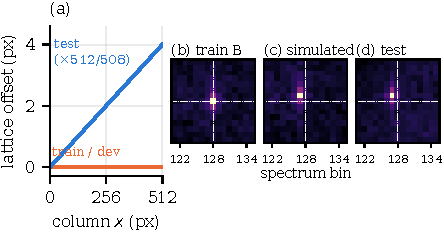
\includegraphics[width=\linewidth]{fig/diagnosis.pdf}
  \caption{\textbf{Diagnosis.} (a) Offset of the generators' 8-pixel lattice relative to the image origin along a row. It is constant in training and dev images and drifts by up to 4~px in test images after a $512/508$ stretch. (b--d) Mean log-magnitude spectrum of the high-pass luma around the period-4 diagonal site at bin 128 (dotted lines). The peak sits exactly at 128 for Model~B training images (b) and moves to 127 after our simulated processing (c), matching the real test set (d).}
  \label{fig:diagnosis}
\end{figure}

\subsection{A transformation-robust detector}
\label{sec:v4}
To make the Baseline ResNet model more robust to different distributions and transformations, the followiing changes to the architecture and training were applied:

\noindent\textbf{Anti-aliased down-sampling.} A stride-2 convolution keeps one pixel in four, so its output depends on the input position modulo 2. Stacked over three stages, the features depend on the position modulo 8, exactly the lattice period~\cite{azulay2019small}. In stages 2--4 we replace each stride-2 convolution, and its $1\times1$ shortcut, by a stride-1 convolution followed by BlurPool~\cite{zhang2019blurpool}:
\begin{equation}
  \mathrm{BP}(h) = \big(h * \tfrac{1}{16}[1\;2\;1]^{\top}[1\;2\;1]\big)\!\downarrow_2 .
\end{equation}
BlurPool has no parameters. NPR keeps its $2\times2$ anchoring, so full invariance must still be learnt from data.

\noindent\textbf{Offline augmentation.} We store 10 augmented copies of every training image, and 20 copies for the 25\% of fakes with the least texture (mean absolute luma high-pass), which are the hardest fakes. That gives 140k copies, plus the 12k originals (\cref{fig:overview}a). Each copy passes through a random chain:
(A)~brightness and contrast $\times$[0.8,\,1.2] ($p{=}.5$), saturation $\times$[0.5,\,1.3] (.5), hue $\pm$0.03 (.2), gamma [0.8,\,1.25] (.3), greyscale (.05), and blurring of 1--2 rectangles covering 10--40\% of the image ($\sigma$ 2--5, .2), which teaches the network to rely on whatever texture remains;
(B)~rescaling by a factor in [0.9,\,1.1] with one of five resamplers (.8), a horizontal flip (.5) and a random multiple of $90^\circ$;
(C)~Gaussian blur $\sigma\in$[0.3,\,0.8] (.1), noise $\sigma\in$[1,\,3] (.1), and JPEG q60--100 with random 4:4:4/4:2:2/4:2:0 sub-sampling (.8, re-encoded twice in 20\% of cases).
The ranges were set after the diagnosis. They \emph{cover} the type of processing observed, with a wide margin, rather than reproduce it: the factor 1.008 is one point in a 20\%-wide interval, and q90 4:2:0 is one of about 120 JPEG settings. Storing the copies (18\,GB) keeps JPEG and resampling out of the training loop and makes every sample reproducible.

\noindent\textbf{Crop training, full-image testing.} Training draws one random $256^2$ crop per stored image. Crops cover all lattice phases and carry less scene content. The network is fully convolutional, so test images are processed whole. We train for 30 epochs with AdamW (lr $2\cdot10^{-3}$, weight decay $10^{-2}$, one epoch of linear warm-up, then cosine decay), a batch of 256 on 8 GPUs, and mixed precision. One epoch over 152k crops takes about 135\,s.

\noindent\textbf{Validation and selection.} On the 3,000 held-out images, which have no stored copies, we track three numbers: \emph{clean} accuracy, \emph{simulated-test} accuracy (\cref{sec:diagnosis}), and \emph{harsh} accuracy (the training augmentation with a fixed seed, centre $448^2$ crop). The checkpoint is selected on harsh accuracy, not on the simulator. Dev is an independent check only. Its labels are the baseline's dev predictions, which the leaderboard scored at 100\%.
